\documentclass{article}
\usepackage{amsfonts}
\usepackage{graphicx}



\title{
{\large{Univerza v Ljubljani}}\\ 
{\large{Fakulteta za matematiko in fiziko}}\\ 
{\large{Univerzitetni študijski progra Finančna matematika}}\\ 
\vspace{5cm}
{\textbf{Pareto fronte v več dimenzijah}
\vspace{5cm}}
}

\author{Klara Penko, Nejc Jenko}
\date{Januar 2022}


\begin{document}

\begin{titlepage}
    \maketitle
\end{titlepage}

\section{Uvod}
V projektni nalogi si bova ogledala Pareto fronte na d-dimenzionalnih množicah. To pomeni, da bova na podani množici poiskala točke, ki so nedominirane. Celotna množica nedominiranih točk je Pareto fronta.  Za opazovane množice točk bova vzela poljubne točke v d-dimenzionalnih kroglah in hiperkockah. Analizirala bova, število točk v Pareto fronti, glede na dimenzijo prostora d. Poleg prve Pareto fronte, bova želela izračunati še drugo, tretjo in tako naprej.

\section{Definicija Pareto fronte}
${\rm \textbf{Definicija 1}}$ Naj bo S prostor definiran z množico n dimenzij $\{d_{1},d_{2}\dots,d_{n}\}$ in D podmnožica množice S. Naj bo $p \in D$, podana z $p = (p_{1},p_{2},\dots,p_{n})$, kjer je $p_{i}$ vrednost v dimenziji $d_{i}$. Točka $p \in D$ \textbf{dominira} točko $q \in D$ na podprostoru $S'\subseteq S$, če v vsaki dimenziji $d_{i} \in S'$ velja $p_{i} \le q_{i}$ in v vsaj eni dimenziji $d_{j} \in S'$, $p_{j} < q_{j}$. 
\underline{\textbf{Pareto fronta}} prostora $S' \subseteq S$ je množica točk $D' \subseteq D,$ ki niso dominirane z nobeno točko v prostoru $S'$. \break
\break

${\rm \textbf{Primer Pareto fronte v dveh dimenzijah}}$

 \begin{figure}[htbp]
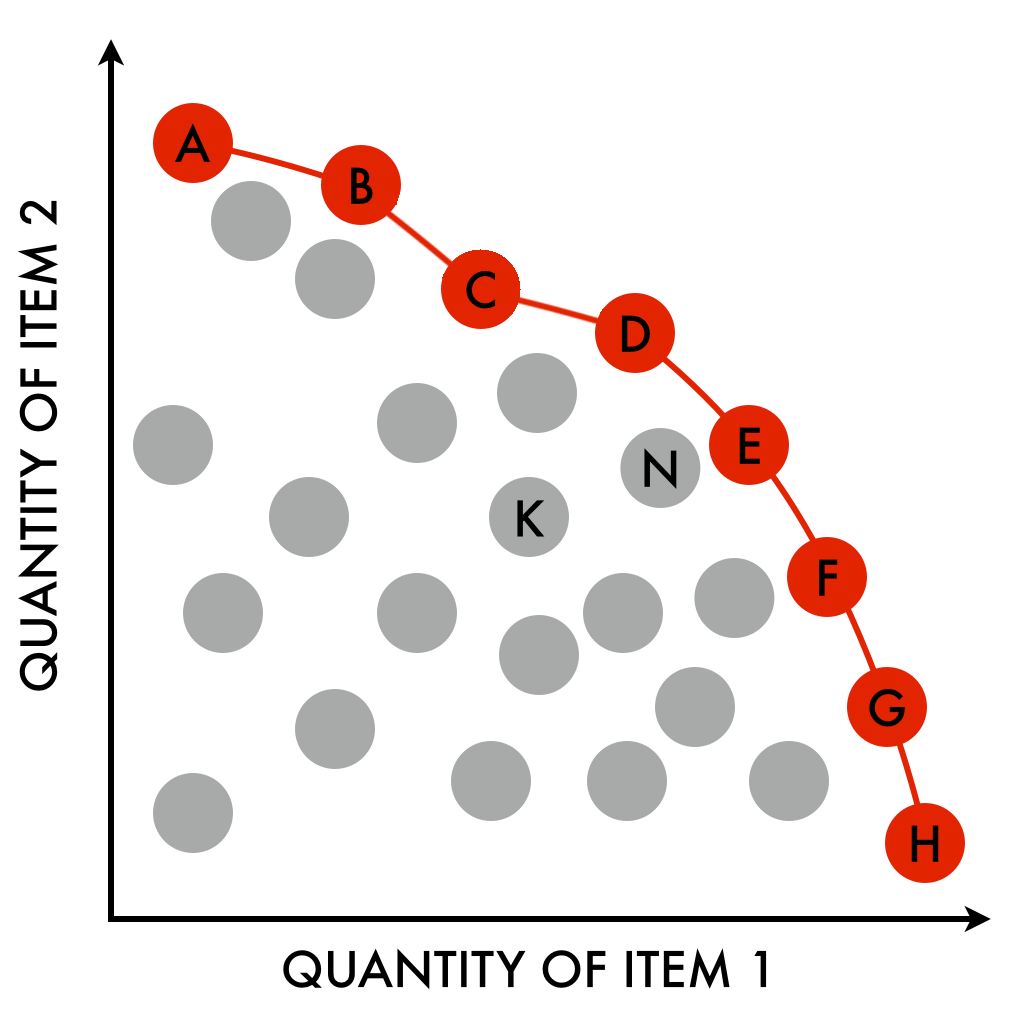
\includegraphics[width=4cm]{Slike/Slika_pareto_fronta.png}
\centering
\end{figure}

\section{Potek dela}
Za generiranje najinega problema sva uporabila programski jezik Python. Glavni vhodni podatek problema je poljubna množica točk, ki jo lahko ročno izberemo sami, ali pa jo dobimo s pomočjo ene od funkcij, ki sva jih zapisala za generiranje le teh. Zapisala sva funkcijo za izračun Pareto fronte, za katero sva dodatno definirala še eno krajšo funkcijo, kot bomo videli v nadaljevanju. Poleg tega sva zapisala funkciji za generiranje točk v d- dimenzionalni krogli in hiperkocki.

\subsection{Funkcije za izračun Pareto fronte}

Glavna funkcija najine projektne naloge je funkcija \textbf{izracun\_pareto\_fronte}, ki sprejme množico točki in vrne pareto fronto, ter množico dominiranih točk. Vmes pa se v kodi te funkcije pojavi še funkcija \textbf{dominira}. Koda obeh je zapisana spodaj.

\begin{verbatim}

def dominira(a, b):
    return sum([a[x] >= b[x] for x in range(len(b))]) == len(b)
\end{verbatim}

Ta funkcija sprejme dve točki(poljubne iste dimenzije) in vrne \textbf{True}, če točka a dominira točko b. Funkcijo \textbf{dominira} uporabimo v naslednji kodi.

\begin{verbatim}

def izracun_pareto_fronte(mnozica): 
    pareto_fronta = set()
    dominirane_tocke = set()

    while len(mnozica) != 0:
        kandidat = list(mnozica)[0] 
        mnozica.remove(kandidat)
        i = 0
        ni_dominirana = True 

        while i < len(mnozica):
            tocka = list(mnozica)[i]
            if dominira(kandidat, tocka): 
                mnozica.remove(tocka)
                dominirane_tocke.add(tuple(tocka))
            elif dominira(tocka, kandidat):
                dominirane_tocke.add(tuple(kandidat))
                ni_dominirana = False
                break
            else:
                i += 1

        if ni_dominirana:   
            pareto_fronta.add(tuple(kandidat))
        
    return pareto_fronta, dominirane_tocke

  
\end{verbatim}

V zgornji fuknciji najprej določimo prazne množice za iskano množico Pareto fronta in iskano množico dominiranih točk. Najprej si iz množice, ki jo podamo funkciji izberemo prvega kandidata in ga odstranimi iz prvotne množice. Za tega preverimo ali ta dominira točke, ki so še ostale v množici oziroma če katera od točk iz množice dominira izbranega kandidata. V primeru, da kandidat dominira točko, jo dodamo v množico, ki nam bo vrnila dominirane točke.  Ta postopek ponavljamo dokler, ne pregledamo vseh točk iz podane množice (tj. podana množica je prazna). Tako nam zapisana funkcija vrne iskano Pareto fronto, ter množico dominiranih točk.


\subsection{Funkcija za izračun n pareto front}
Poleg računanja prve Pareto fronte, sva se lotila pisanja kode za funkcijo, ki bo vrnila n Pareto front. Spodnja funkcija, kot argument sprejme poljubno množico točk, ter število n. S številom n povemo koliko Pareto front, bi želeli izračunati. Pareto fronte, tukaj izračunamo rekurzivno s pomočjo zgoraj definirane fukncije izracun\_pareto\_fronte. Množico zmanjšujemo, dokler ne pridemo do željene Pareto fronte oziroma dokler ne izpraznimo podane možice točk.

\begin{verbatim}
def izracun_n_pareto_front(mnozica, n): 
    if len(mnozica) == 0:   
        return set()
    elif n < 1:
        return set()    
    else:
        pareto, dom = izracun_pareto_fronte(mnozica)
        print(len(pareto))  
        return pareto, izracun_n_pareto_front(dom, n-1)
\end{verbatim}

\subsection{Funkcija za generiranje točk na d-dimenzionalni enotski krogli}
Funkciji \textbf{random\_krogla} podamo število točk, ki jih želimo zgenerirati in dimenzijo prostora, dodatno lahko spremenimo tudi parameter radij, če bi gledali neenotske krogle (tj. radij krogle različen od 1). V kodi najprej zgeneriramo naključni vektor dimenzije d in ga normiramo. Dobljeni vektor pomnožimo z naključno vrednostjo med 0 in 1, da dobimo točko v notranjosti d dimenzionalne krogle. Na ta način zgeneriramo toliko točk, kot smo podali z atributom stevilo\_tock.
\begin{verbatim}
def random_krogla(stevilo_tock, d, radij=1):
    mnozica_tock = set()
    for i in range(stevilo_tock):    
        rand_smer = random.uniform(low=-1, high=1, size=d) 
        rand_smer /= linalg.norm(rand_smer, axis=0) 
        rand_dolzina = random.uniform(low=0, high=1) 
        tocka = tuple(radij * (rand_smer * rand_dolzina)) 
        mnozica_tock.add(tocka)
    return mnozica_tock
\end{verbatim}


\subsection{Funkcija za generiranje točk na hiperkocki s stranico a}
Podobno, kot smo zgenerirali točke znotraj enotske d-dimenzionalne krogle, zdaj zgeneriramo točke znotraj hiperkocke. Funkciji podamo število točk, dimenzijo prostori in stranico hiperkocke a. Če stranice ne podamo, funkcija privzeto zgenerira točke v enotski hiperkocki. V kodi zgeneriramo naključen vektor velikosti d, z vrednostmi med 0 in a, kar nam predstavlja eno točko. In tako zgeneriramo toliko točk kot smo podali.
\begin{verbatim}
def random_kocka(stevilo_tock,d,a=1): 
    mnozica_tock = set()
    for i in range(stevilo_tock):
        rand_smer = random.uniform(low=0, high=a, size=d)
        tocka = tuple(rand_smer)
        mnozica_tock.add(tocka)
    return mnozica_tock
\end{verbatim}





\section{Eksperimentalni Del}
Ko imamo napisane funkcije za generiranje podatkov in njihovo obdelavo, lahko začnemo z eksperimentalnim delom. 
V prvem delu bomo za svoje podatke generirali 2, 3, 4 in 5 dimenzionalne krogle in primerjali število točk v prvih petih pareto forntah. Za vsako dimenzijo bomo opazovali množice po 50, 100 in 200 točk. Za vsako od teh kombinacij bomo poskus ponovili desetkrat. 
\



\end{document}